\section{Introduction}
% \begin{itemize}
% $    \item P1: Succeeding in the long-horizon manipulation tasks require to retreive past information: highlight different types of information that can be retrieved: temporal, spatial, numerical, sequential, event-time, motor information to solve different task. Solutions tailored towards one specific type is not good.
% $    \item P2: Learning to retrieve past information directly from data provides a general mechanism. A recipe successul in language and vision domains
% $    \item P3: However, extending this approach to imitation learning in robotic systems introduces two key challenges:
% $        \subitem Encouraging each decision to be based on retrieved task-relevant information, rather than on spurious correlations between past observations and current actions
% $        \subitem Limiting the influence of accumulated errors during retrieval, arising from prediction errors that propagate via closed-loop interaction with the environment
% $    \item P4: Our approach:
% $        \subitem We use knowledge distillation from foundation models to provide priors on what information to retrieve and how to query it, steering the policy toward task-relevant information
% $        \subitem To mitigate drift in closed-loop execution, we control information flow via Top-K sparsification, forcing the policy to focus on a small set of the most important signals at each step, thereby reducing error accumulation
% $    \item P5: Results
% General-purpose robots operating in household environments must solve long-horizon manipulation tasks under partial observability, where task-relevant information is often no longer present in the current sensory input.
% \end{itemize}
% General-purpose robots operating in household environments must solve long-horizon manipulation tasks that require recalling relevant information no longer present in current sensory input.
% Examples include remembering where an object was placed, when the appliance was turned on, how many pieces of bread were placed in the oven, or which sub-tasks have already been completed (Fig.~\ref{fig:pull_figure}).
% As a result, purely reactive visuomotor policies will fail on such tasks, motivating the need for mechanisms that allow them to retrieve and use the information from earlier in the episode.
\begin{figure}[htbp]
    \centering
    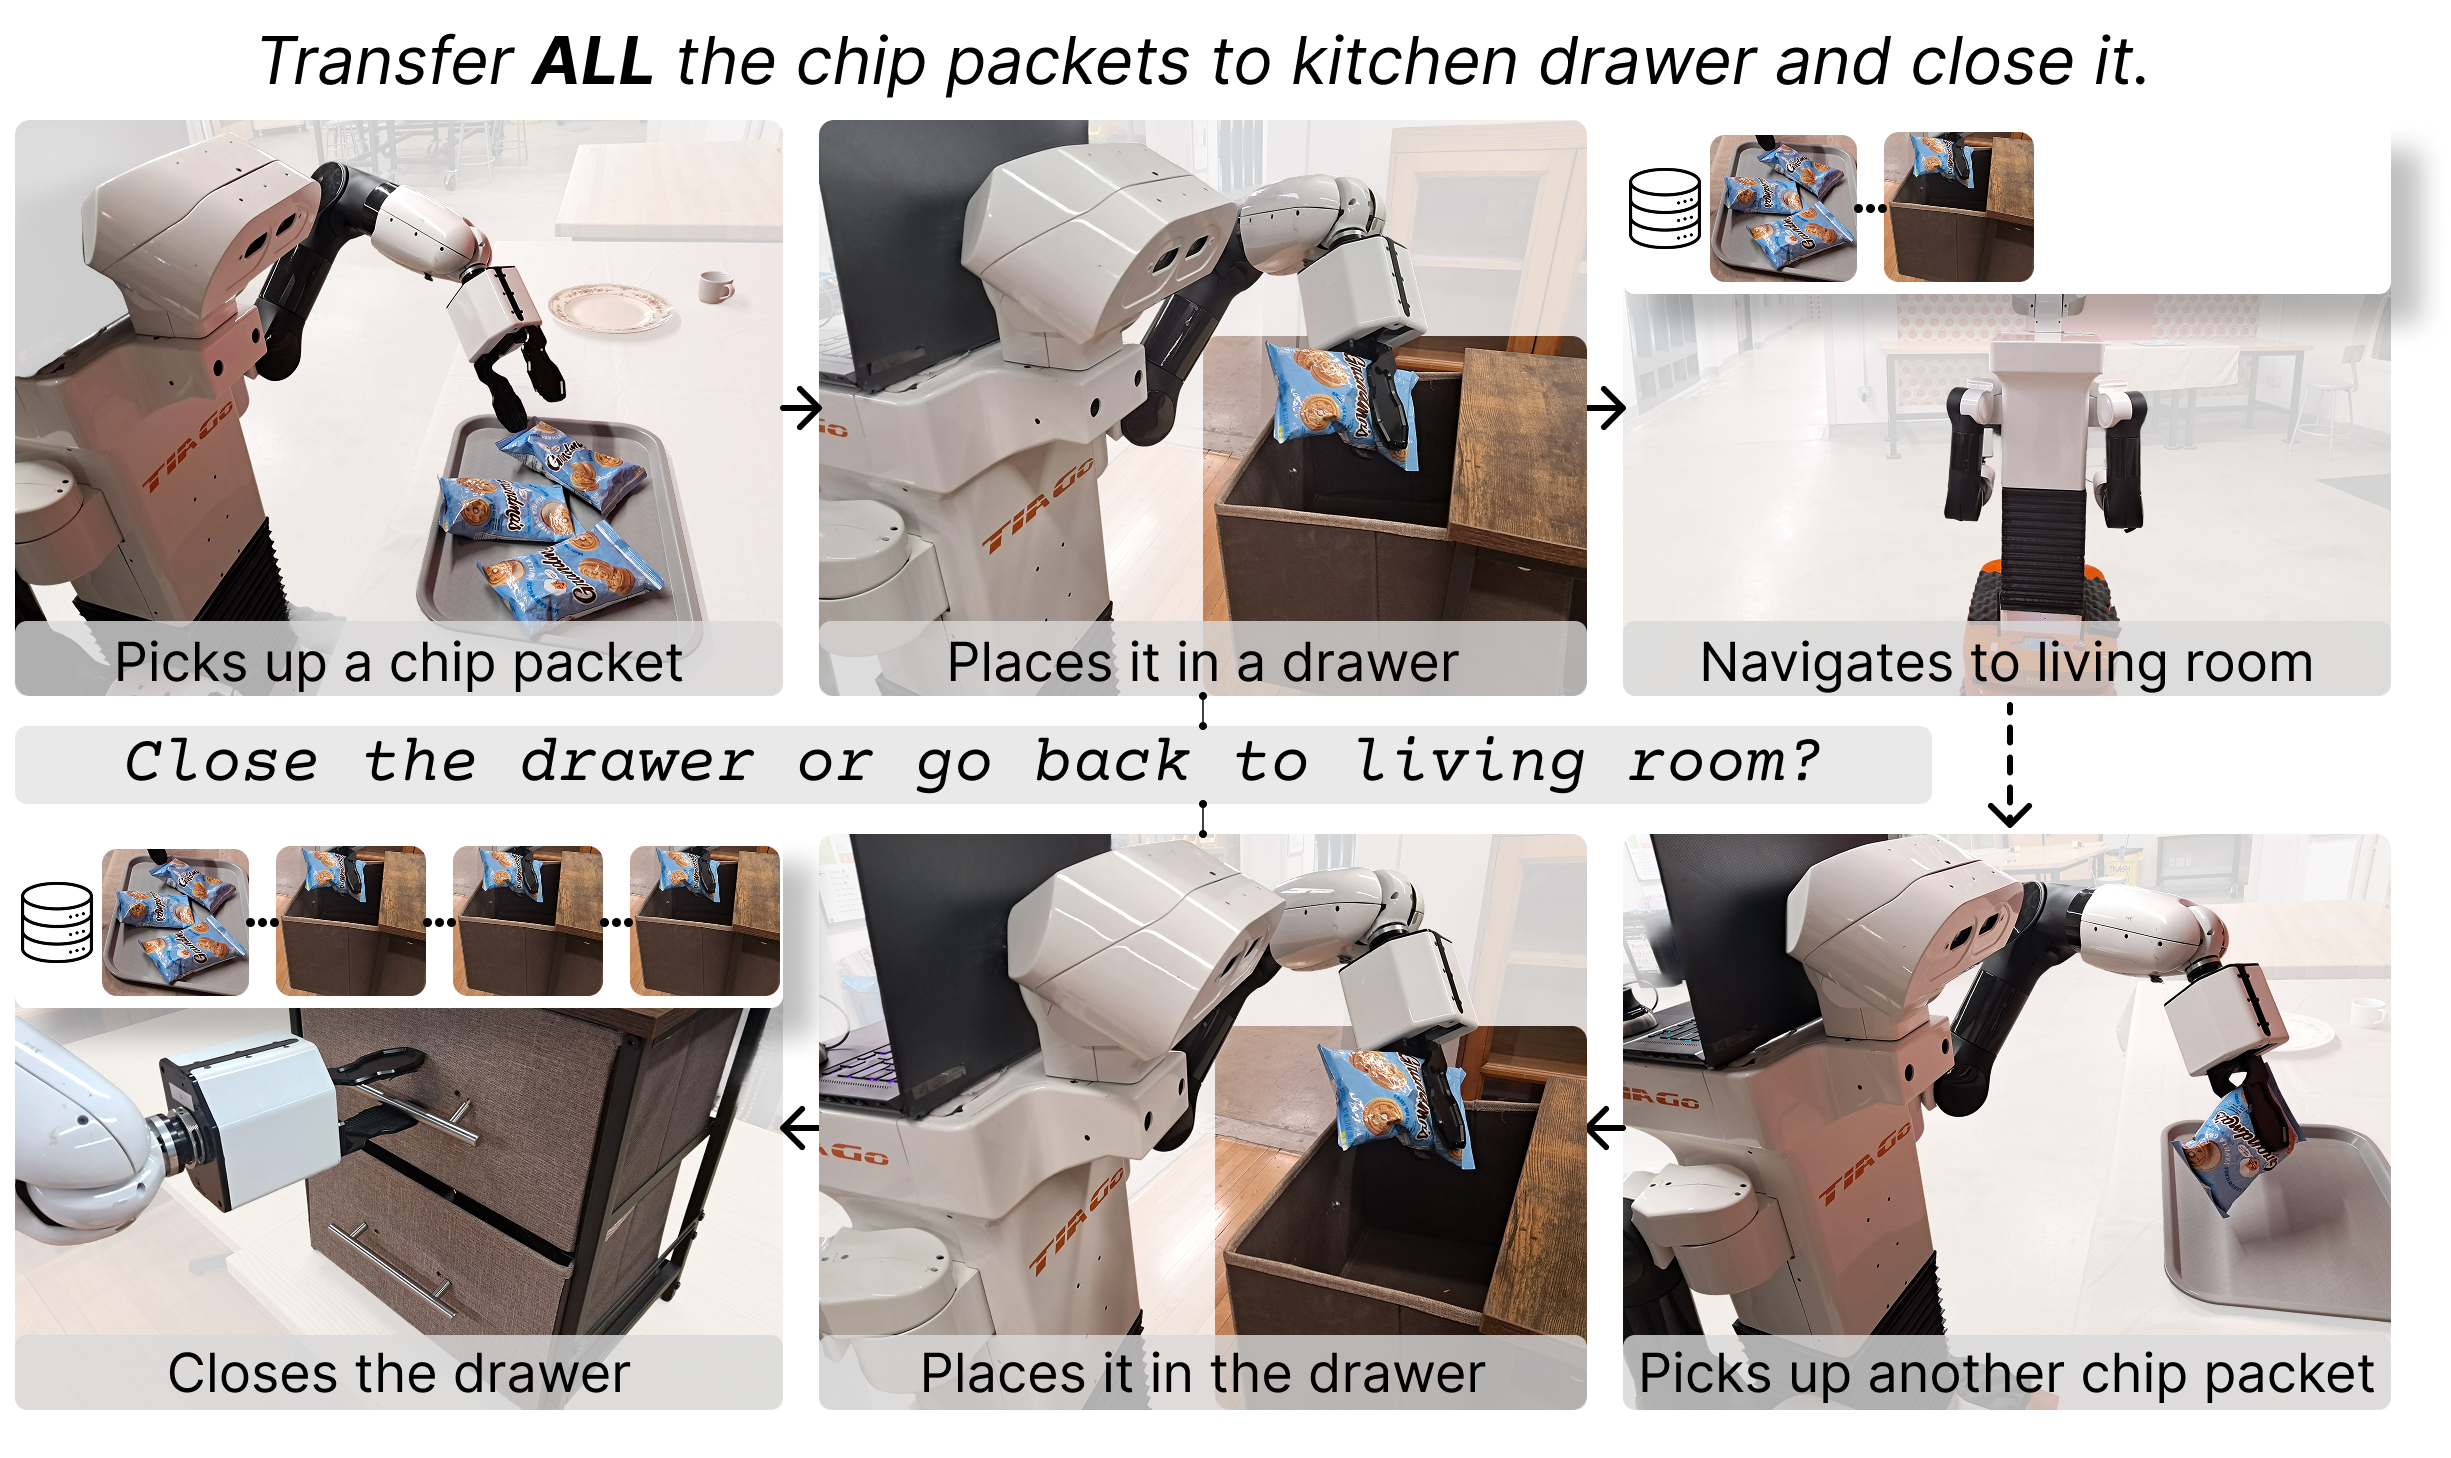
\includegraphics[width=0.5\textwidth, trim=0 0.5cm 0 0, clip]{figures/pull_figurev3.png}
    \vspace{-20pt}
    \caption{\textbf{Memory retrieval in visuomotor policy learning.} Long-horizon household tasks require robots to act on information no longer present in the current sensory input. Under partial observability, the policy must retrieve relevant information from past observations stored in memory to predict correct low-level actions. The type of information needed can change across task stages, motivating a general, learned retrieval mechanism.}
    \label{fig:pull_figure}
    \vspace{-10pt}
\end{figure}

General-purpose robots operating in household environments must solve long-horizon manipulation tasks that require recalling information no longer present in current sensory input.
The robot may need to remember where an object was placed earlier, when an appliance was turned on, how many pieces of bread were placed in the oven, or which tasks have already been completed (Fig.~\ref{fig:pull_figure}).
Such requirements arise frequently in everyday household activities, where successfully completing the task depends on recalling information over extended time horizons.
As a result, purely reactive visuomotor policies will fail on these tasks, motivating the need for \textbf{memory retrieval} mechanisms that can leverage information gathered earlier~\cite{tulving1972episodic,atkinson1968human}.

The information that robots must recall from history is diverse.
It may include spatial information such as object locations, relational information between objects, numerical quantities, temporal events, or event ordering.
Approaches based on hand-designed memory representations or modality-specific retrieval rules, therefore, struggle to scale across the wide range of manipulation tasks required of general-purpose robots~\cite{guadarrama2014open, clipnav, sam2act}.
This motivates the development of a \textit{general} memory retrieval mechanism that can be learned end-to-end, rather than tailored to individual tasks or modalities~\cite{sukhbaatar2015end,graves2014neural,graves2016hybrid,lstm}.
%Crucially, different tasks may depend on different combinations of these information types. 

Among candidate mechanisms for general memory retrieval, associative retrieval based on learned query-key similarity, such as attention in transformers, has emerged as a promising mechanism~\cite{carpenter1989neural,vaswani2017attention}.
By learning both queries and keys from data, associative retrieval avoids modality-specific design, and has demonstrated strong empirical performance in domains such as language processing~\cite{floridi2020gpt}.
However, directly applying attention-based memory retrieval to long-horizon robotic imitation learning via offline data exposes two fundamental challenges.
First, policies may exploit spurious correlations between past observations and current actions, \textit{i.e.}, attending to information that correlates with expert behavior in the training data but is not causally relevant to task execution.
\begin{figure}[htbp]
    \centering
    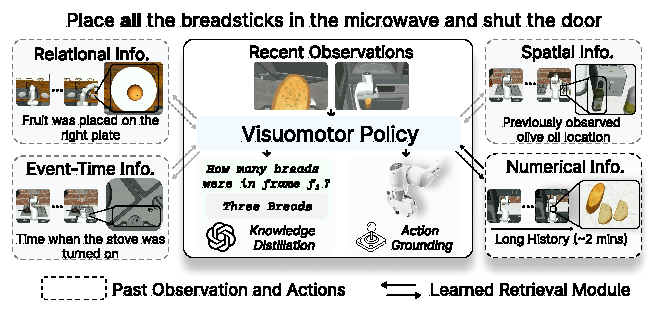
\includegraphics[width=0.5\textwidth]{figures/pull_figure_halo.pdf}
    \vspace{-20pt}
    \caption{\ourmethod{} learns to retrieve diverse forms of task-relevant information from history, guided by priors distilled from vision-language foundation models.}
    \label{fig:overview}
    \vspace{-10pt}
\end{figure}
Such correlations often fail to hold at test time, leading to poor performance~\cite{de2019causal,wen2020fighting}.
Second, in offline imitation learning, small prediction errors compound during closed-loop online execution~\cite{ross2011reduction,spencer2021feedback}. 
Conditioning on large amounts of past observations can amplify this effect, as the policy repeatedly attends to noisy information, leading to drift and cascading failures over long horizons.
Together, these challenges can limit the effective use of memory in imitation learning, a crucial capability for partially observable long-horizon tasks.

To address these challenges, we propose \ourmethod{}: \textbf{H}istory-\textbf{A}ware visuomotor policy for \textbf{LO}ng-horizon robotic imitation learning.
Our key insight is that while attention provides a general retrieval mechanism, it must be guided towards task-relevant information and constrained to avoid conditioning on irrelevant or noisy history (Fig.~\ref{fig:overview}).


To mitigate spurious correlations, we build on the observation that vision-language models (VLMs) encode rich priors about which information from past observations is relevant for a task~\cite{bubeck2023sparks}.
Although these priors are not grounded in action and are therefore insufficient on their own for control, they provide useful signals for identifying task-relevant information in history.
In \ourmethod{}, we distill these priors into the policy through automatically generated video question–answer (VQA) supervision.
To answer these questions correctly, the retrieval module must attend to specific parts of the history where task-relevant event(s) occurred, providing direct supervision on what should be retrieved from memory.
The policy is co-trained to both imitate expert actions and answer questions about past observations. The VQA objective biases memory retrieval towards task-relevant information, whereas the action prediction objective may still access information needed for low-level control.
This contrasts with prior work that incorporates VLM priors through text-based summaries~\cite{anwar2025remembr}, which may omit details needed for low-level control.

To address error accumulation over long horizons, \ourmethod{} further restricts the policy to condition only on a sparse subset of stored information.
Rather than attending to the full history, the policy retrieves the top-$k$ most informative observations or actions via learned query-key matching and conditions exclusively in these elements~\cite{child2019generating}. 
This explicit sparsification limits the incorporation of noisy information, reducing closed-loop drift and mitigating cascading failures during execution.

We evaluate our approach on \textsc{ReMemBench}~\cite{anonymous2026scaling}, a benchmark for long-horizon manipulation tasks that require diverse forms of memory, as well as on five real-world tasks across two robotic platforms, including a fixed-base manipulator and a mobile manipulator.
Across these settings, we show that VQA-induced task priors provide a general solution, improving absolute task success by $7\%$ on average across diverse tasks and outperforming prior methods based on hand-designed rules ($-12\%$) and task-specific features ($-21\%$).
We further find that while vision-language models encode informative priors about task-relevant information, policies using these priors alone reach only $18\%$ absolute success, compared to $41\%$ with action-grounded retrieval, highlighting the importance of grounding retrieval in action prediction.
In addition, we demonstrate that top-$k$ attention sparsification improves absolute performance by $10\%$, reducing model drift, and outperforms alternative memory mechanisms based on memory compression by $29\%$.
Together, these results highlight the importance of learning to retrieve task-relevant information from memory and grounding retrieval in action prediction for long-horizon control.
%Through qualitative analysis, we show that \ourmethod{} reduces spurious correlations between task-irrelevant past observations and predicted actions via VQA induced-priors.
%Finally, we identified our failure modes across tasks and provided insights to guide future work on robotic policies with a memory retrieval mechanism.


% First, we leverage knowledge in foundation models to provide priors on which information to retrieve, biasing the policy toward task-relevant context and reducing spurious correlations.
% We distill this prior into the policy using automatically generated video question-answer (VQA) supervision that directly guides the retrieval process.
% The policy is co-trained with VQA supervision and a behavioral cloning loss derived from expert teleoperation demonstrations. Co-training allows the policy to be guided by priors from vision-language foundation models while ensuring it remains grounded in task-relevant action prediction.
% To further mitigate error accumulation during closed-loop execution, we regulate the information flow via Top-$K$ sparsification, ensuring each decision depends only on the most relevant information. 
% This explicit sparsification reduces the effect of error accumulation.
% We further compare against other auxiliary tasks that improve recall, including past-action prediction and masked video modeling, and find consistent gains from the knowledge embedded in foundation models.
%  \\
%  \rutav{
%  Method Names Brainstorming:
%  \\ \\
%  HALO (long-\textbf{H}orizon m\textbf{A}nipu\textbf{L}ation using retrieval-augmented visu\textbf{O}motor policy)
%  \\ \\
%  ECHO (l\textbf{E}arning to retrieve for \textbf{C}losed-loop, long-\textbf{HO}rizon control)
%  }
